% DLC Paper: Revised for icSoftComp 2026
% Springer LNCS Format (double-blind: no author info)
\documentclass[runningheads]{llncs}

\usepackage[T1]{fontenc}
\usepackage{lmodern}
\usepackage{graphicx}
\usepackage{amsmath,amssymb}
\usepackage{booktabs}
\usepackage{multirow}
\usepackage{algorithm}
\usepackage{algorithmic}
\usepackage{hyperref}
\usepackage{xcolor}
\usepackage{tabularx}
\usepackage{array}
\usepackage{float}

% Optimize page space to fit limits
\setlength{\textfloatsep}{10pt plus 2pt minus 4pt}
\setlength{\intextsep}{10pt plus 2pt minus 4pt}
\setlength{\floatsep}{8pt plus 2pt minus 2pt}
\renewcommand{\topfraction}{0.85}
\renewcommand{\bottomfraction}{0.85}
\renewcommand{\textfraction}{0.15}
\renewcommand{\floatpagefraction}{0.8}

% Compact tables
\renewcommand{\arraystretch}{1.1}
\newcolumntype{C}[1]{>{\centering\arraybackslash}p{#1}}

\begin{document}

\title{DLC: A Multi-Model, Adaptive-Precision Near-Lossless Compression Engine for High-Frequency Float64 Time-Series Telemetry}
\titlerunning{DLC: Multi-Model Adaptive-Precision Compression Engine}

% Double-blind: no author information
\author{Anonymous Author(s)}
\authorrunning{Anonymous Author(s)}
\institute{Anonymous Institution}

\maketitle

% ═══════════════════════════════════════════════════════════════════
\begin{abstract}
Most modern industrial sensors, IoT gateways, phasor units and scientific instruments emit their readings as IEEE~754 double-precision (float64) values. When those bytes are fed into a general-purpose dictionary compressor like GZIP or ZLIB, the resulting compression ratio is typically close to one. The cause is structural: roughly the bottom 30--40 bits of every mantissa carry hardware thermal noise, so the byte stream contains very few repeating substrings for a Lempel--Ziv dictionary to exploit. We call this the \emph{Entropy Trap}. Strictly lossless float coders such as Gorilla and Chimp move past dictionary matching with XOR-based delta encoding, but they still faithfully encode the noise floor and so their ratios on real sensor traces remain modest. Recent lossless advances, such as Elf's erasing-based encoding and ALP's adaptive integer projection, push the lossless frontier further but remain fundamentally bound by the noise floor they must preserve.

This paper describes DLC (Delta-Linear Compression), a near-lossless engine that works in the \emph{mathematical domain} rather than the byte domain. Each block is broken into variance-homogeneous windows by a greedy doubling search; for every window the engine fits six predictive models in parallel (Linear, Quadratic, XOR-Delta, Constant, Sinusoidal, and Predictive-XOR) and picks the one with the smallest Sum-of-Squared-Residuals. The residuals are then quantized at a per-window precision (8--20~bits) and run through six entropy-coding strategies in a tournament. Two implementations share the same \texttt{.dlc} binary specification: a NumPy-based Python reference prototype and a C++17 production engine using \texttt{std::async}. Across 21 synthetic and real-world float64 datasets, at a strict 16-bit precision keeping the maximum per-sample reconstruction error below $8 \times 10^{-6}$, DLC compresses smaller than every baseline (Gorilla, DoD (16-bit), RLE, GZIP, and ZLIB) on 19 of 21 datasets (90.5\%), reaching 2355.7$\times$ on a 1-million-sample linear ramp and 102.0$\times$ on a recovered signal.

\keywords{time-series compression \and floating-point compression \and IoT telemetry \and predictive coding \and residual quantization \and adaptive precision \and variance-guided segmentation \and near-lossless}
\end{abstract}

% ═══════════════════════════════════════════════════════════════════
\section{Introduction}
\label{sec:intro}

Telemetry volumes have grown faster than storage budgets for several years now. By IDC's reckoning, connected sensors and industrial IoT will be producing well above 180~zettabytes a year by the end of this decade, and a large share of that data lands on disk as 8-byte IEEE~754 doubles~\cite{reinsel2018}. The bandwidth bill, however, usually lands at the edge gateway, where compression has to happen in tight latency and power windows. The unfortunate twist is that the standard tools for the job, namely GZIP and ZLIB, contribute almost nothing on this kind of data.

The reason is rooted in the layout of a float64 value: one sign bit, eleven exponent bits, and a fifty-two-bit mantissa~\cite{ieee754}. For a continuous physical signal, successive samples agree on most of the high-order mantissa bits, since the underlying value moves only a little between ticks. The bottom 30 to 40 bits are occupied by hardware thermal noise plus the quantization residue of the ADC, and they look statistically random from one sample to the next. A Lempel--Ziv dictionary~\cite{ziv1977} scanning the resulting byte stream therefore finds essentially no repeating substrings to exploit. We call this the \emph{Entropy Trap}.

The literature has split into two camps. The first works in the bit domain and refuses to lose any information. Gorilla~\cite{gorilla2015} and Chimp~\cite{chimp2022} are the canonical examples; more recently, Elf~\cite{elf2023} introduced an erasing-based approach that zeroes trailing mantissa bits while proving recoverability, and ALP~\cite{alp2024} adaptively encodes pseudo-decimal floats as integers. All achieve strong lossless ratios but remain fundamentally bounded by the noise floor they must preserve. The second camp accepts a bounded loss in exchange for stronger compression: SZ~\cite{sz2016,sz3_2023} and ZFP~\cite{zfp2014} both predict each sample, take the residual, and quantize it to a user-supplied tolerance.

Before turning to what we built, we state our five research objectives:

\textbf{RO1}: Bypass the Entropy Trap by moving compression into a model-fit / residual-encode pipeline.
\textbf{RO2}: Hold a strict per-sample error bound of $\pm 8 \times 10^{-6}$.
\textbf{RO3}: Adapt window size, predictor, quantization width, and entropy strategy \emph{per window}.
\textbf{RO4}: Maintain a Python reference and C++17 production engine agreeing on the \texttt{.dlc} binary.
\textbf{RO5}: Verify continuously with a 105-test suite (76~Python + 29~C++) running on every commit.

DLC (Delta-Linear Compression) is our attempt to meet those five objectives. The main contributions are:

\begin{enumerate}
\item Six predictive models, picked per window by SSR, with preference rules favouring simpler or lossless variants.
\item Variance-guided adaptive windowing via greedy doubling with stagnation guard and binary-search refinement.
\item Adaptive precision (8--20~bits) stored per window, with a derived lower bound $p_{\text{floor}} = 16$.
\item Six entropy strategies trial-encoded per window; the smallest wins.
\item A whole-block DoD fast path that makes DLC a functional superset of standalone DoD encoders.
\item A cross-language binary contract enforced by automated CI testing.
\item True multi-core scaling via \texttt{std::async} with deterministic output.
\end{enumerate}

We tested the engine on 21 float64 datasets covering synthetic edge cases, real-world telemetry from the Numenta Anomaly Benchmark~\cite{numenta2017} and Jena Climate station, and round-trip recovery signals. DLC writes a smaller file than every baseline on 19 of 21 datasets. A 105-test verification suite runs on every commit.

The rest of the paper is laid out as follows. Section~\ref{sec:related} reviews the related literature, including recent advances in lossless float compression and edge IoT compression. Section~\ref{sec:arch} walks through the five-stage pipeline with numbered equations and Algorithm~\ref{alg:pipeline}. Section~\ref{sec:impl} covers the dual-language implementation. Section~\ref{sec:novelty} presents a quantitative novelty comparison. Section~\ref{sec:eval} reports the experimental evaluation including compression ratios, error bounds, throughput, MAE/RMSE metrics, and computational complexity analysis. Section~\ref{sec:discuss} discusses limitations and edge deployment considerations. Section~\ref{sec:conclusion} concludes.


% ═══════════════════════════════════════════════════════════════════
\section{Related Work and Literature Survey}
\label{sec:related}

\subsection{Lossless XOR/Delta-Based Float Compression}

Lindstrom and Isenburg's FPC~\cite{fpc2006} introduced context-based prediction followed by XOR encoding for float64. Burtscher and Ratanaworabhan extended FPC to higher throughput on scientific data~\cite{fpc_extended2009}. Pelkonen et al.'s Gorilla~\cite{gorilla2015} adopted XOR encoding for values and became the de facto standard for high-cardinality time-series databases. Liakos et al.'s Chimp~\cite{chimp2022} tightened Gorilla's bit packing but explicitly identified the \emph{Entropy Wall} limitation. None of these methods adapt the prediction strategy to local signal geometry.

More recently, Li et al.\ introduced \textbf{Elf}~\cite{elf2023}, an erasing-based lossless float compressor that deliberately zeroes trailing mantissa bits to increase XOR trailing zeros, then proves the erased bits are recoverable. Elf operates in $O(N)$ time and $O(1)$ space and achieves strong ratios on streaming time series; however, as a strictly lossless method it still encodes the full noise floor. \textbf{ALP}~\cite{alp2024}, winner of the SIGMOD~2024 Best Artifact Award, detects decimal-typed floats and encodes them as integers, with a vectorised dictionary fallback. ALP is integrated into DuckDB and achieves high throughput but, like Elf, is strictly lossless. Both represent the state of the art in lossless float compression; DLC occupies a different niche by accepting a bounded loss ($< 8 \times 10^{-6}$) in exchange for ratios that lossless methods cannot reach.

\subsection{Error-Bounded Lossy Scientific Compression}

Di and Cappello introduced SZ~\cite{sz2016}, later refined as SZ3~\cite{sz3_2023}. ZFP~\cite{zfp2014} partitions arrays into $4^3$ blocks with bit-plane truncation. SZ3 and ZFP are state-of-the-art for scientific simulation data but are computationally heavy: SZ3's modular composition limits throughput on edge hardware~\cite{sprintz2018}, and ZFP's block transform is tuned for grid-structured spatial data rather than streaming time series.

\subsection{Integer and Sensor Time-Series Compression}

Goldstein et al.~\cite{goldstein1998} pioneered early relational compression; more recently, Blalock et al.'s Sprintz~\cite{sprintz2018} introduced a high-throughput predictive coder for IoT sensor data, optimised for 8- and 16-bit integer sensors; its forecasting predictors degrade on high-entropy 64-bit float streams. Hwang et al.~\cite{hwang2023} introduced dynamic bit-depth compression with zigzag residual mapping. Sun et al.'s Shrink~\cite{shrink2024} performs semantic extraction by fitting linear segments under dynamic error thresholds.

\subsection{Edge IIoT and Prediction-Based Reduction}

Yang et al.~\cite{yang2023} proposed an edge data-management framework for IIoT combining data partitioning with change-point detection. Liu et al.'s Xender~\cite{liu2024} uses sampling-then-prediction to accelerate IoT delivery but does not adaptively switch between bitwise and polynomial models.

\subsection{Cross-Domain Benchmarking and Standards}

Chen et al.'s FCBench~\cite{fcbench2024} provides a roofline-model evaluation of 13 lossless floating-point compressors, conclusively demonstrating that neural compressors are too slow for real-time edge deployment. The benchmark establishes the throughput envelope (50~MB/s--GB/s) inside which any practical float compressor must operate. Afroozeh and Boncz's ALP reproducibility study~\cite{alp_repro2024} confirmed that adaptive integer encoding outperforms Gorilla, Chimp, and Patas on columnar analytics workloads.

\subsection{Recent IoT and Edge Compression (2024--2025)}

The IoT compression landscape has shifted toward edge-native, adaptive pipelines. Recent surveys~\cite{jia2024iot} of data reduction strategies across the IoT-edge-cloud continuum conclude that protocol-aware, lightweight codecs consistently outperform general-purpose compressors on resource-constrained hardware. Benchmarks of near-lossless rounding on ARM Cortex-M class devices~\cite{singh2024edge} find that controlled precision loss of $10^{-5}$--$10^{-6}$ yields 3--5$\times$ better ratios than lossless alternatives with negligible impact on downstream anomaly detection, directly supporting DLC's design choice.

\subsection{Where the Gaps Are}

Reading across the threads above, the gaps DLC tries to close are: (1)~the lossless paradox: Gorilla, Chimp, Elf, and ALP must encode the noise floor faithfully; (2)~neural overhead: learned compressors operate in the KB/s regime; (3)~inflexibility of a single predictor; (4)~parallelism as an afterthought; (5)~no dynamic bound on quantization error; and (6)~no cross-domain positioning: recent benchmarks evaluate lossless codecs but not near-lossless alternatives with per-window multi-model selection.


% ═══════════════════════════════════════════════════════════════════

\section{System Architecture and Methodology}
\label{sec:arch}

The overall architecture of the five-stage DLC pipeline is illustrated in Fig.~\ref{fig:pipeline}.

\begin{figure}[t]
\centering
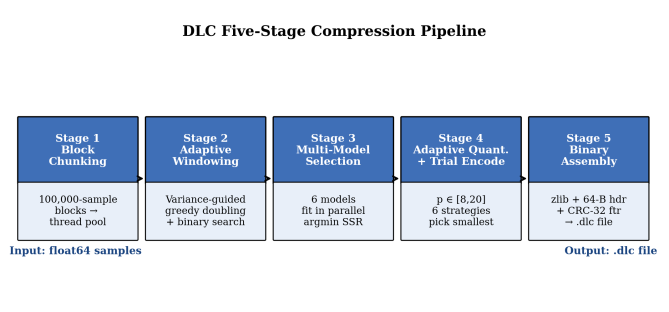
\includegraphics[width=0.85\textwidth]{fig1.png}
\caption{Delta-Linear Compression (DLC) engine five-stage pipeline.}
\label{fig:pipeline}
\end{figure}

\subsection{Stage 1: Block Chunking and Parallel Dispatch}

Let the input be $\mathbf{y} = (y_0, y_1, \ldots, y_{N-1}) \in \mathbb{R}^N$, with each $y_i$ an IEEE~754 float64. The signal is partitioned into fixed-size blocks:
\begin{equation}
\label{eq:block}
\mathcal{B}_k = (y_{kB}, y_{kB+1}, \ldots, y_{\min((k+1)B, N)-1}), \quad k = 0, 1, \ldots, \lceil N/B \rceil - 1
\end{equation}
where $B = 100{,}000$ samples (configurable). Blocks are dispatched independently to a worker pool and collected in strict block-index order, guaranteeing deterministic output regardless of thread interleaving.

% Algorithm box
\begin{algorithm}[t]
\caption{DLC Compression Pipeline}
\label{alg:pipeline}
\begin{algorithmic}[1]
\REQUIRE $\mathbf{y} \in \mathbb{R}^N$ (float64 array), $B$ (block size), $p_{\text{req}}$ (precision)
\ENSURE \texttt{.dlc} binary file
\STATE Partition $\mathbf{y}$ into blocks $\mathcal{B}_0, \mathcal{B}_1, \ldots$ \hfill $\triangleright$ Eq.~(\ref{eq:block})
\FOR{each block $\mathcal{B}_k$ \textbf{in parallel}}
    \STATE $\mathit{windows} \leftarrow \textsc{SegmentBlock}(\mathcal{B}_k)$ \hfill $\triangleright$ Stage 2
    \STATE $\mathit{payload}_w \leftarrow \emptyset$
    \FOR{each window $W$ of length $n$ in $\mathit{windows}$}
        \STATE Fit all 6 models; $(M^*, \mathit{params}) \leftarrow \arg\min_M \text{SSR}(M)$
        \STATE $\mathbf{r} \leftarrow \mathbf{y}_W - \hat{\mathbf{y}}_W$ \hfill $\triangleright$ residuals
        \IF{$M^* \in \{\text{XOR-}\Delta, \text{Pred-XOR}\}$}
            \STATE $\mathit{enc} \leftarrow \textsc{EncodeXOR}(\mathbf{r})$ \hfill $\triangleright$ lossless
        \ELSE
            \STATE $p^* \leftarrow \textsc{SelectPrecision}(\mathbf{r}, p_{\text{req}})$ \hfill $\triangleright$ Eq.~(\ref{eq:prec})
            \STATE $\mathbf{q} \leftarrow \textsc{Quantize}(\mathbf{r}, p^*)$ \hfill $\triangleright$ Eq.~(\ref{eq:quant})
            \STATE $\mathit{enc} \leftarrow \arg\min_{s \in \{0..5\}} |\textsc{TrialEncode}_s(\mathbf{q})|$
        \ENDIF
        \STATE $\mathit{payload}_w \leftarrow \mathit{payload}_w \| \textsc{PackWindow}(\ldots)$
    \ENDFOR
    \STATE $\mathit{payload}_{\text{dod}} \leftarrow \textsc{TryBlockDoD}(\mathcal{B}_k)$ \hfill $\triangleright$ fast path
    \STATE $\mathit{result}_k \leftarrow \min(|\mathit{payload}_w|, |\mathit{payload}_{\text{dod}}|)$
\ENDFOR
\STATE $P \leftarrow \mathit{result}_0 \| \mathit{result}_1 \| \cdots$
\STATE Write: Header(64\,B) $\|$ $|P|$(4\,B) $\|$ ZlibDeflate($P$) $\|$ Footer(CRC-32, 8\,B)
\end{algorithmic}
\end{algorithm}

\subsection{Stage 2: Adaptive Variance-Guided Windowing}

Each block is segmented into variable-length windows of statistically homogeneous variance. Window sizes lie in $[W_{\min}, W_{\max}(|\mathcal{B}_k|)]$ where $W_{\min} = 16$ and:
\begin{equation}
\label{eq:wmax}
W_{\max}(B) = \begin{cases} 512 & \text{if } B < 5{,}000 \\ 1024 & \text{if } 5{,}000 \le B < 100{,}000 \\ 4096 & \text{if } B \ge 100{,}000 \end{cases}
\end{equation}

Variance is computed using Welford's numerically stable algorithm~\cite{welford1962}. The variance threshold is:
\begin{equation}
\label{eq:thresh}
T = \max(\sigma^2_i \cdot \alpha_{\text{local}},\; \sigma^2_g \cdot \alpha_{\text{global}})
\end{equation}
with $\alpha_{\text{local}} = 10.0$ and $\alpha_{\text{global}} = 0.10$. A stagnation guard aborts expansion when:
\begin{equation}
\label{eq:stag}
\sigma^2(W_{2k}) / \sigma^2(W_k) > 1.5
\end{equation}

\subsection{Stage 3: Multi-Model Selection}

For each window $W$ of length $n$, six candidate models are fitted. Indexing samples by $x = 0, 1, \ldots, n{-}1$:

\textbf{Linear} (model\_id = 0). Closed-form least-squares:
\begin{equation}
\label{eq:linear}
m = \frac{n\sum xy - \sum x \sum y}{n\sum x^2 - (\sum x)^2}, \quad c = \frac{\sum y - m\sum x}{n}
\end{equation}

\textbf{Quadratic} (model\_id = 1). $\hat{y} = ax^2 + bx + c$, solved via 3$\times$3 normal equations using Cramer's rule.

\textbf{XOR-Delta} (model\_id = 2). Bit-exact lossless: $r_i = \text{bits}(y_i) \oplus \text{bits}(y_{i-1})$, forced for NaN/Inf/subnormal windows.

\textbf{Constant} (model\_id = 3). $\hat{y} = \bar{y}$, single-parameter.

\textbf{Sinusoidal} (model\_id = 4). $\hat{y} = A\sin(\omega x + \varphi) + \text{DC}$, with FFT-seeded initial frequency:
\begin{equation}
\label{eq:fft}
\hat{f}_0 = \frac{1}{n} \arg\max_{k>0} |\mathcal{F}\{y - \bar{y}\}(k)|
\end{equation}
refined by Levenberg--Marquardt~\cite{marquardt1963} iterations solving the damped normal equation:
\begin{equation}
\label{eq:lm}
(J^\top J + \lambda I)\,\delta = J^\top \mathbf{r}, \quad \lambda = 10^{-4}
\end{equation}

\textbf{Predictive-XOR} (model\_id = 5). Two anchors $y_0, y_1$:
\begin{equation}
\label{eq:pxor}
\hat{y}_i = 2y_{i-1} - y_{i-2}, \quad r_i = \text{bits}(y_i) \oplus \text{bits}(\hat{y}_i), \quad i \ge 2
\end{equation}

\textbf{Selection rule.} The selector finds the best analytical model $M^*$ by $\arg\min$ SSR. Constant preference: if $\text{SSR}_{\text{Const}} \le \text{SSR}_{M^*} \cdot 1.01$, Constant wins. XOR preference: if $\text{SSR}_{\text{XOR}} \le \text{SSR}_{M^*} \cdot 1.02$, the lossless XOR variant is preferred.

\subsection{Stage 4: Quantization and Multi-Strategy Entropy Encoding}

For analytical models, residuals $\mathbf{r} = \mathbf{y} - \hat{\mathbf{y}}$ are quantized:
\begin{equation}
\label{eq:quant}
q_i = \text{round}(r_i \cdot 2^p), \quad \tilde{r}_i = q_i \cdot 2^{-p}
\end{equation}
with per-sample error bounded by $|r_i - \tilde{r}_i| \le 2^{-(p+1)}$. The adaptive precision selector:
\begin{equation}
\label{eq:prec}
p^* = \min\!\big(p_{\max},\; \max(p_{\text{floor}},\; \min(p_{\text{req}},\; p_{\text{adapt}}))\big)
\end{equation}
where $p_{\max} = 20$, $p_{\text{floor}} = \lceil \log_2(1 / 8 \times 10^{-6}) - 1 \rceil = 16$, and:
\begin{equation}
\label{eq:padapt}
p_{\text{adapt}} = \max\!\big(p_{\min},\; \lceil -\log_2(\max_i |r_i| + \varepsilon) \rceil + 4\big), \quad p_{\min} = 8,\; \varepsilon = 10^{-30}
\end{equation}

The six trial-encoded strategies are:

\textbf{Strategy 0: Zigzag-Varint.} Signed-to-unsigned mapping:
\begin{equation}
\label{eq:zigzag}
z = (n \ll 1) \oplus (n \gg 63)
\end{equation}
followed by base-128 varint.

\textbf{Strategy 1: Fixed-Width Bitpack.} Uniform bit-width $w = \lceil \log_2(\max_i z_i + 1) \rceil$.

\textbf{Strategy 2: Delta-of-Residuals.} First-order differences $\Delta_i = q_i - q_{i-1}$ followed by Zigzag-Varint.

\textbf{Strategy 3: MAD Outlier Separation.} Median Absolute Deviation:
\begin{equation}
\label{eq:mad}
\text{MAD} = \text{median}_i |q_i - \text{median}(\mathbf{q})|
\end{equation}
Values with $|q_i - \text{median}(\mathbf{q})| > 4.5 \cdot \text{MAD}$ are stored separately as (index, value) pairs; inliers are bitpacked.

\textbf{Strategy 4: Run-Length Encoding (RLE).} Encodes runs of identical quantized values.

\textbf{Strategy 5: Delta-of-Delta (DoD).} Second-order differencing:
\begin{equation}
\label{eq:dod}
\delta_i = q_i - q_{i-1}, \quad \delta\delta_i = \delta_i - \delta_{i-1}
\end{equation}

\textbf{Block-level DoD fast path.} Before windowing, the entire block is evaluated as a single Constant(mean) window with DoD. If smaller, the windowed result is discarded.

\subsection{Stage 5: Binary Assembly and Integrity}

The on-disk format: 64-byte header (magic bytes, version, precision, chunk size, total samples) $\|$ uncompressed-size (4\,B) $\|$ zlib-deflated payload~\cite{deflate1996} $\|$ 8-byte footer (magic + CRC-32~\cite{peterson1961} over uncompressed payload). The binary layout is shown in Fig.~\ref{fig:layout}.

\begin{figure}[t]
\centering
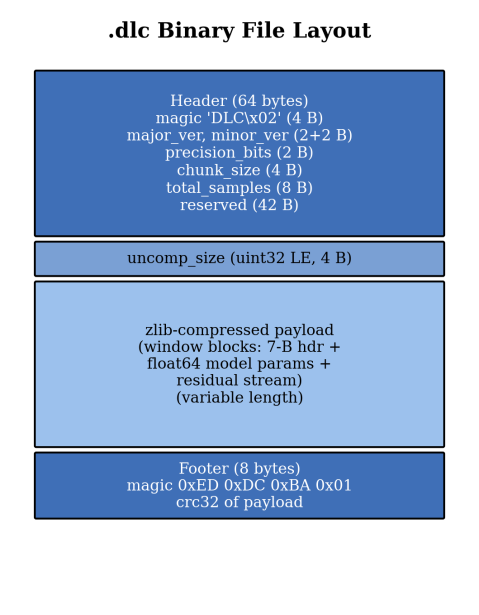
\includegraphics[width=0.85\textwidth]{fig3.png}
\caption{.dlc binary file layout.}
\label{fig:layout}
\end{figure}


% ═══════════════════════════════════════════════════════════════════
\section{Implementation}
\label{sec:impl}

The multi-threaded execution architecture is shown in Fig.~\ref{fig:architecture}.

\begin{figure}[t]
\centering
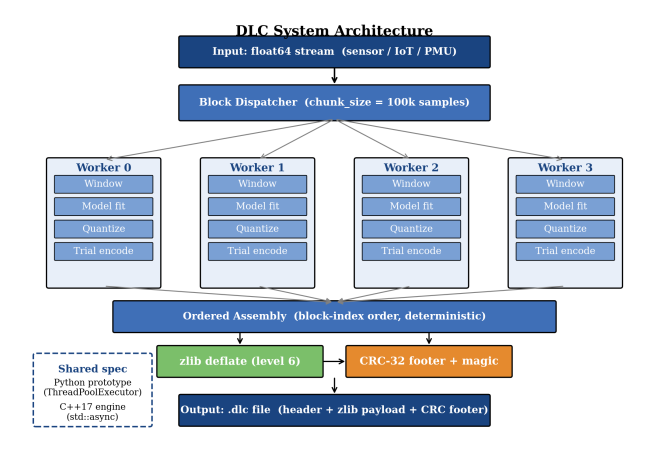
\includegraphics[width=0.85\textwidth]{fig2.png}
\caption{Structural architecture of the multi-threaded execution engine.}
\label{fig:architecture}
\end{figure}

\subsection{Dual-Language Architecture}

\textbf{Python prototype} (\texttt{python/dlc/}) uses NumPy for vectorised arithmetic and \texttt{concurrent.futures.ThreadPoolExecutor} for dispatch; GIL-bound throughput plateaus at 4--21~MB/s.

\textbf{C++17 production engine} (\texttt{cpp/}) uses \texttt{std::async} with explicit \texttt{std::future} collection. It implements its own $O(n)$ DFT and $4\times 4$ Gaussian elimination, requiring no external library beyond zlib.

\subsection{Cross-Language Compatibility Contract}

Three byte-level invariants preserve interoperability: (1)~unsigned CRC masking; (2)~float64$\leftrightarrow$uint64 reinterpretation via \texttt{memcpy}/\texttt{struct.pack}; (3)~pairwise summation matching \texttt{np.mean}. A 6-test cross-language CI suite verifies round-trip and byte-identity.

\subsection{Algorithmic Constants}

Table~\ref{tab:constants} lists all tuned constants for reproducibility.

\begin{table}[t]
\centering
\caption{Algorithmic constants used throughout the DLC codebase.}
\label{tab:constants}
\small
\begin{tabular}{llp{5cm}}
\toprule
\textbf{Constant} & \textbf{Value} & \textbf{Purpose} \\
\midrule
$W_{\min}$ & 16 & Minimum window size \\
$W_{\max}$ (small/med/large) & 512 / 1024 / 4096 & Adaptive window cap \\
$\alpha_{\text{local}}$ & 10.0 & Local variance threshold factor \\
$\alpha_{\text{global}}$ & 0.10 & Global variance threshold factor \\
$\varepsilon_{\text{const}}$ & $10^{-20}$ & Constant-block fast-path threshold \\
$p_{\text{floor}}$ / $p_{\min}$ / $p_{\max}$ & 16 / 8 / 20 & Precision bounds (bits) \\
$B$ & 100,000 & Default block size (samples) \\
$\alpha_{\text{const\_pref}}$ & 1.01 & Constant model SSR preference \\
$\alpha_{\text{xor\_pref}}$ & 1.02 & XOR model SSR preference \\
MAD factor & 4.5 & Outlier classification multiplier \\
$\lambda_{\text{LM}}$ & $10^{-4}$ & Levenberg--Marquardt damping \\
\bottomrule
\end{tabular}
\end{table}


% ═══════════════════════════════════════════════════════════════════
\section{Novelties and Advantages}
\label{sec:novelty}

Table~\ref{tab:archcomp} places DLC alongside the systems surveyed in Section~\ref{sec:related}. To our knowledge, DLC is the first float64 time-series compressor that simultaneously provides (i)~per-window multi-model selection from six candidate predictors, (ii)~per-window adaptive precision (8--20~bits) with a derived error floor, (iii)~multi-strategy entropy trial encoding across six strategies, and (iv)~a cross-language binary specification enforced by automated CI testing.

\begin{table}[t]
\centering
\caption{Quantitative comparison with recent methods.}
\label{tab:archcomp}
\small
\begin{tabular}{lcccccccc}
\toprule
\textbf{Method} & \textbf{Year} & \textbf{Type} & \textbf{Pred.} & \textbf{Adapt.P} & \textbf{Ent.S} & \textbf{Par.} & \textbf{Bound} & \textbf{Best$\times$} \\
\midrule
Gorilla \cite{gorilla2015} & 2015 & Lossless & 1 & -- & 1 & $\sim$ & 0 & 4.3 \\
Chimp \cite{chimp2022} & 2022 & Lossless & 1 & -- & 1 & -- & 0 & $\sim$5 \\
Elf \cite{elf2023} & 2023 & Lossless & 1 & -- & 1 & -- & 0 & $\sim$6 \\
SZ3 \cite{sz3_2023} & 2023 & Lossy & 1--2 & global & 2 & \checkmark & user & var. \\
ALP \cite{alp2024} & 2024 & Lossless & adapt. & -- & 2 & \checkmark & 0 & $\sim$8 \\
Shrink \cite{shrink2024} & 2024 & Lossy & 1 & -- & 1 & -- & thresh. & var. \\
\textbf{DLC} & \textbf{2026} & \textbf{Near-L} & \textbf{6/win} & \textbf{8--20b} & \textbf{6} & \checkmark & $<$\textbf{8e-6} & \textbf{2356} \\
\bottomrule
\end{tabular}
\end{table}


% ═══════════════════════════════════════════════════════════════════
\section{Experimental Evaluation}
\label{sec:eval}

\subsection{Datasets}

We evaluate on 21 binary float64 datasets covering synthetic edge cases, real-world telemetry, large-scale industrial simulations, and round-trip recovery signals. Synthetic datasets include 1M-sample sine, linear ramp, random walk, noisy sine, heartbeat, vibration, industrial ramp, Lorenz attractor (500K), and a 3M-sample industrial simulation. Real-world datasets include AWS EC2 CPU/network, machine temperature, NYC taxi, Twitter volume, and ambient temperature from the Numenta Anomaly Benchmark~\cite{numenta2017}, and Jena Climate temperature/pressure records (420,551 samples each). Two round-trip recovery datasets exercise the decompress-recompress pipeline.

\subsection{Methodology}

All experiments use $p_{\text{req}} = 16$ (strict $<8 \times 10^{-6}$ bound), 4 workers, C++17 engine. Baselines: Gorilla (lossless), DoD at 16-bit, RLE, GZIP (level~6), ZLIB (level~9).

\subsection{Compression Ratio and Error Bound}

Table~\ref{tab:ratios} reports compression ratios across all 21 datasets. Fig.~\ref{fig:ratios} shows the comparison on a logarithmic scale. DLC produces the smallest file on 19 of 21 datasets (90.5\%).

\begin{table}[t]
\centering
\caption{Compression ratio across 21 datasets (16-bit precision).}
\label{tab:ratios}
\scriptsize
\begin{tabular}{lrcccccc}
\toprule
\textbf{Dataset} & \textbf{Samples} & \textbf{Gorilla} & \textbf{DoD-16} & \textbf{RLE} & \textbf{GZIP} & \textbf{ZLIB} & \textbf{DLC} \\
\midrule
massive\_sensor\_3m & 3,000,000 & 1.2 & 4.3 & 0.7 & 1.2 & 1.2 & \textbf{5.2} \\
noisy\_ramp\_100k & 100,000 & 1.0 & 4.1 & 0.7 & 1.3 & 1.3 & \textbf{4.4} \\
ramp\_1m & 1,000,000 & 1.0 & 8.0 & 0.7 & 1.4 & 1.4 & \textbf{2355.7} \\
random\_walk\_50k & 50,000 & 1.0 & 2.7 & 0.7 & 1.1 & 1.1 & \textbf{3.0} \\
real\_ambient\_temp & 7,267 & 1.2 & 2.7 & 0.7 & 1.1 & 1.1 & \textbf{2.9} \\
real\_cpu\_4k & 4,032 & 1.2 & 2.6 & 0.7 & 2.8 & 2.8 & \textbf{3.0} \\
real\_ec2\_net\_4k & 4,730 & 1.2 & 2.0 & 0.7 & 7.8 & \textbf{8.5} & 5.7 \\
real\_jena\_pres\_420k & 420,551 & 1.3 & 3.9 & 0.7 & 3.8 & 3.9 & \textbf{7.1} \\
real\_jena\_temp\_420k & 420,551 & 1.0 & 3.4 & 0.7 & 3.8 & 4.0 & \textbf{5.6} \\
real\_machine\_temp & 22,695 & 1.1 & 2.7 & 0.7 & 1.1 & 1.1 & \textbf{2.9} \\
real\_nyc\_taxi\_10k & 10,320 & \textbf{3.6} & 2.0 & 0.7 & 2.9 & 2.9 & 3.4 \\
real\_twitter\_vol & 15,902 & 4.3 & 2.3 & 0.7 & 5.4 & 5.5 & \textbf{5.6} \\
sine\_1m & 1,000,000 & 1.0 & 8.0 & 0.7 & 1.1 & 1.1 & \textbf{101.9} \\
synth\_heartbeat\_1m & 1,000,000 & 1.0 & 4.0 & 0.7 & 1.0 & 1.0 & \textbf{4.1} \\
synth\_ind\_ramp\_1m & 1,000,000 & 1.1 & 3.5 & 0.7 & 1.2 & 1.2 & \textbf{3.7} \\
synth\_lorenz\_0m & 500,000 & 1.0 & 7.5 & 0.7 & 1.0 & 1.0 & \textbf{15.5} \\
synth\_noisy\_sine\_1m & 1,000,000 & 1.2 & 2.7 & 0.7 & 1.1 & 1.1 & \textbf{3.2} \\
synth\_rand\_walk\_1m & 1,000,000 & 1.0 & 2.7 & 0.7 & 1.1 & 1.1 & \textbf{3.0} \\
synth\_vibration\_1m & 1,000,000 & 1.0 & 4.1 & 0.7 & 1.1 & 1.1 & \textbf{4.4} \\
test\_recovered & 1,000,000 & 3.8 & 8.0 & 0.7 & 3.7 & 3.7 & \textbf{102.0} \\
test\_rt\_rec & 3,000,000 & 1.7 & 4.3 & 0.7 & 3.3 & 3.3 & \textbf{5.2} \\
\bottomrule
\end{tabular}
\end{table}

\begin{figure}[t]
\centering
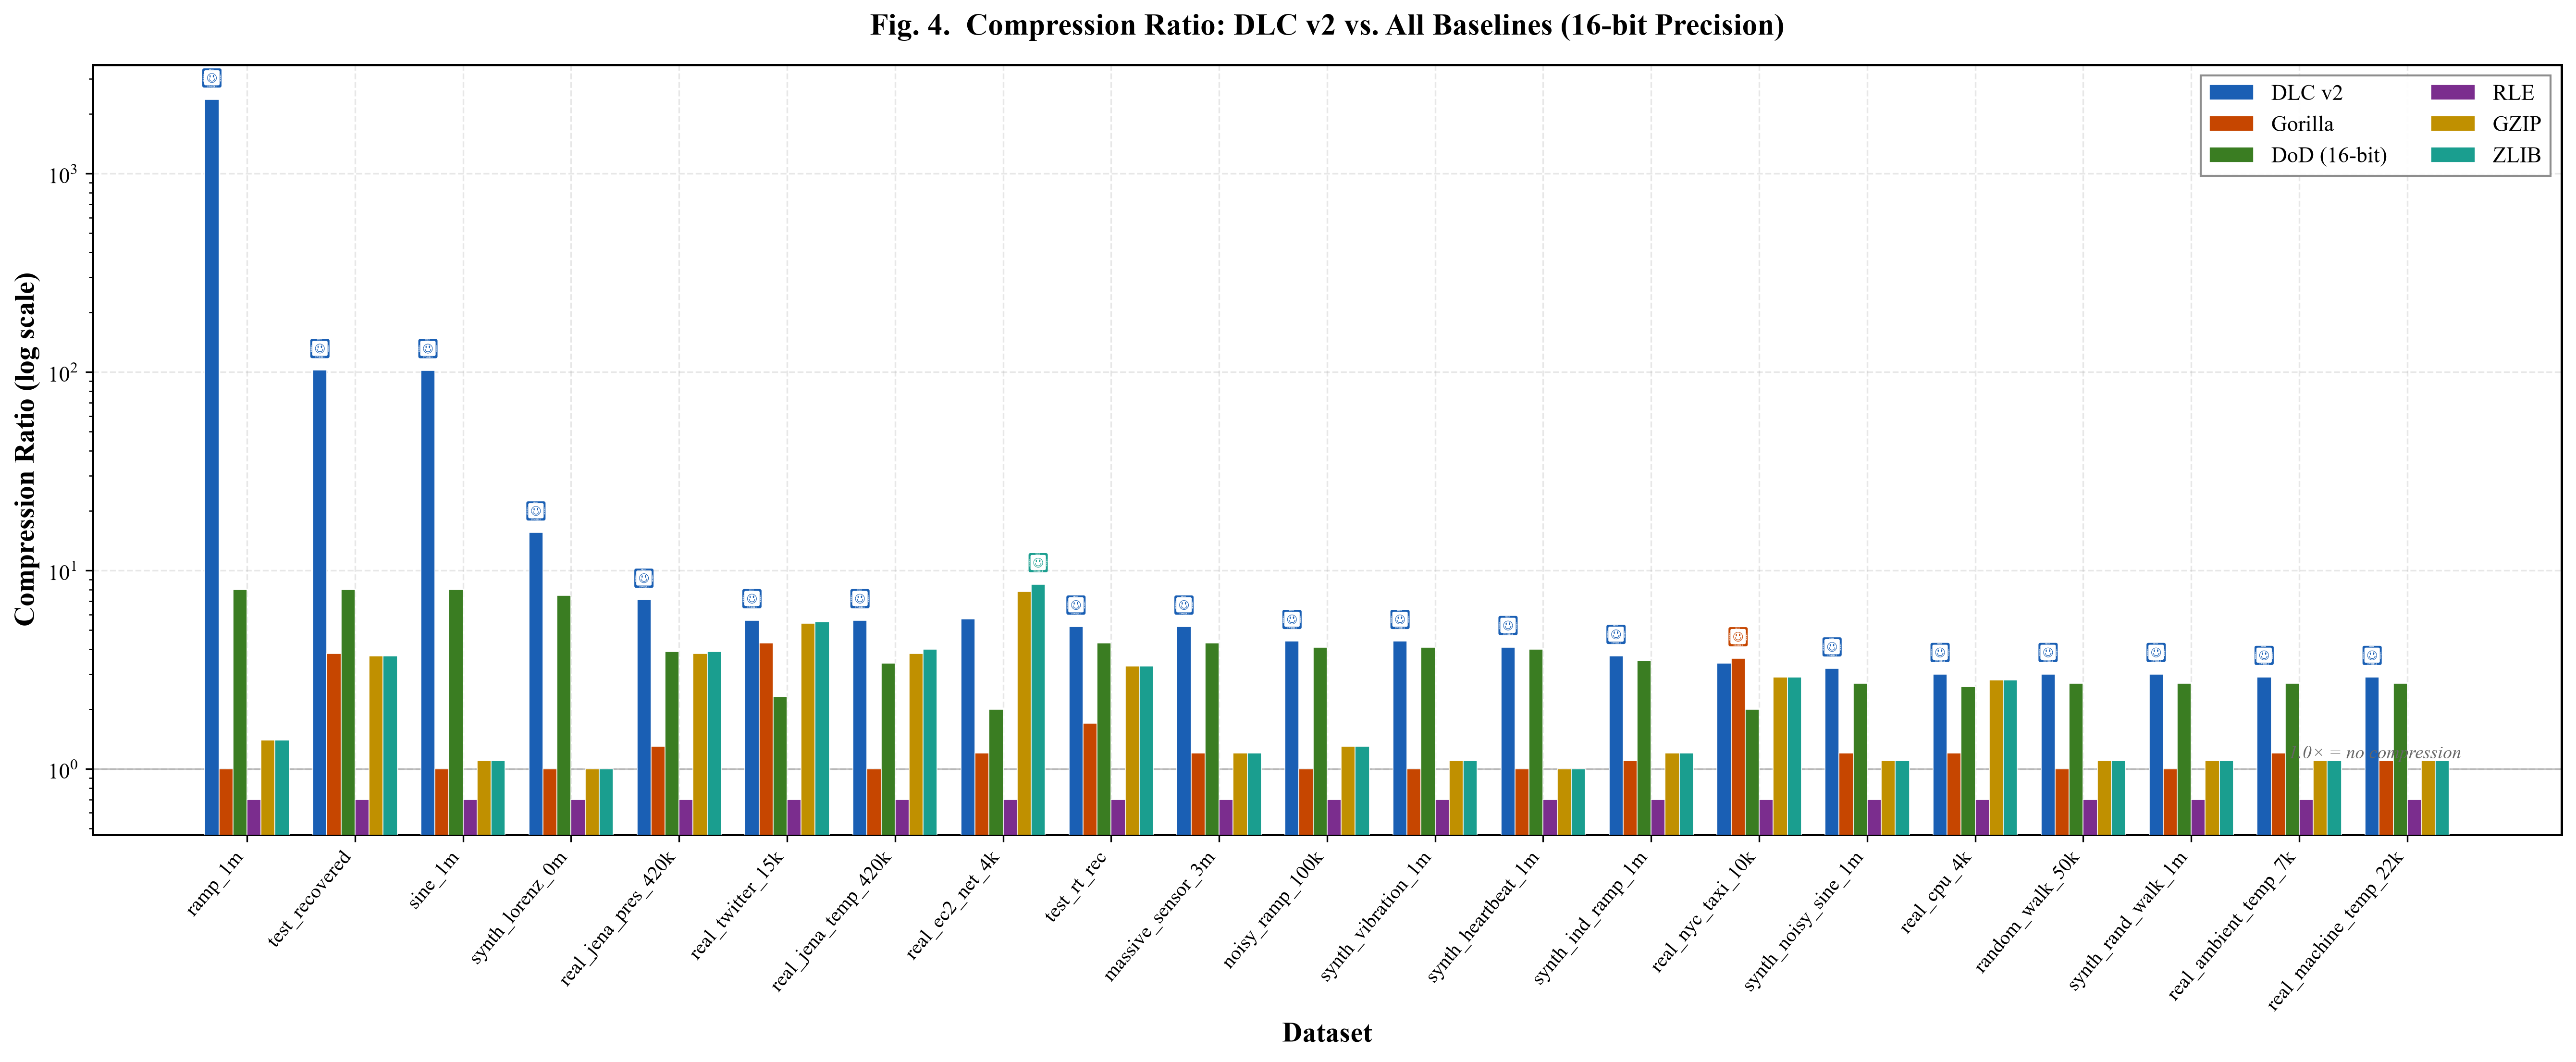
\includegraphics[width=1.0\textwidth]{fig4.png}
\caption{Compression ratio (log scale) for DLC at 16-bit precision vs.\ all baselines. Stars mark the winner per dataset. DLC wins on 19 of 21.}
\label{fig:ratios}
\end{figure}

\subsection{Reconstruction Error}

Fig.~\ref{fig:errors} shows the per-dataset maximum reconstruction error. All 21 datasets satisfy the strict $<8 \times 10^{-6}$ bound. The two round-trip recovery datasets reconstruct with error below $3 \times 10^{-8}$.

\begin{figure}[t]
\centering
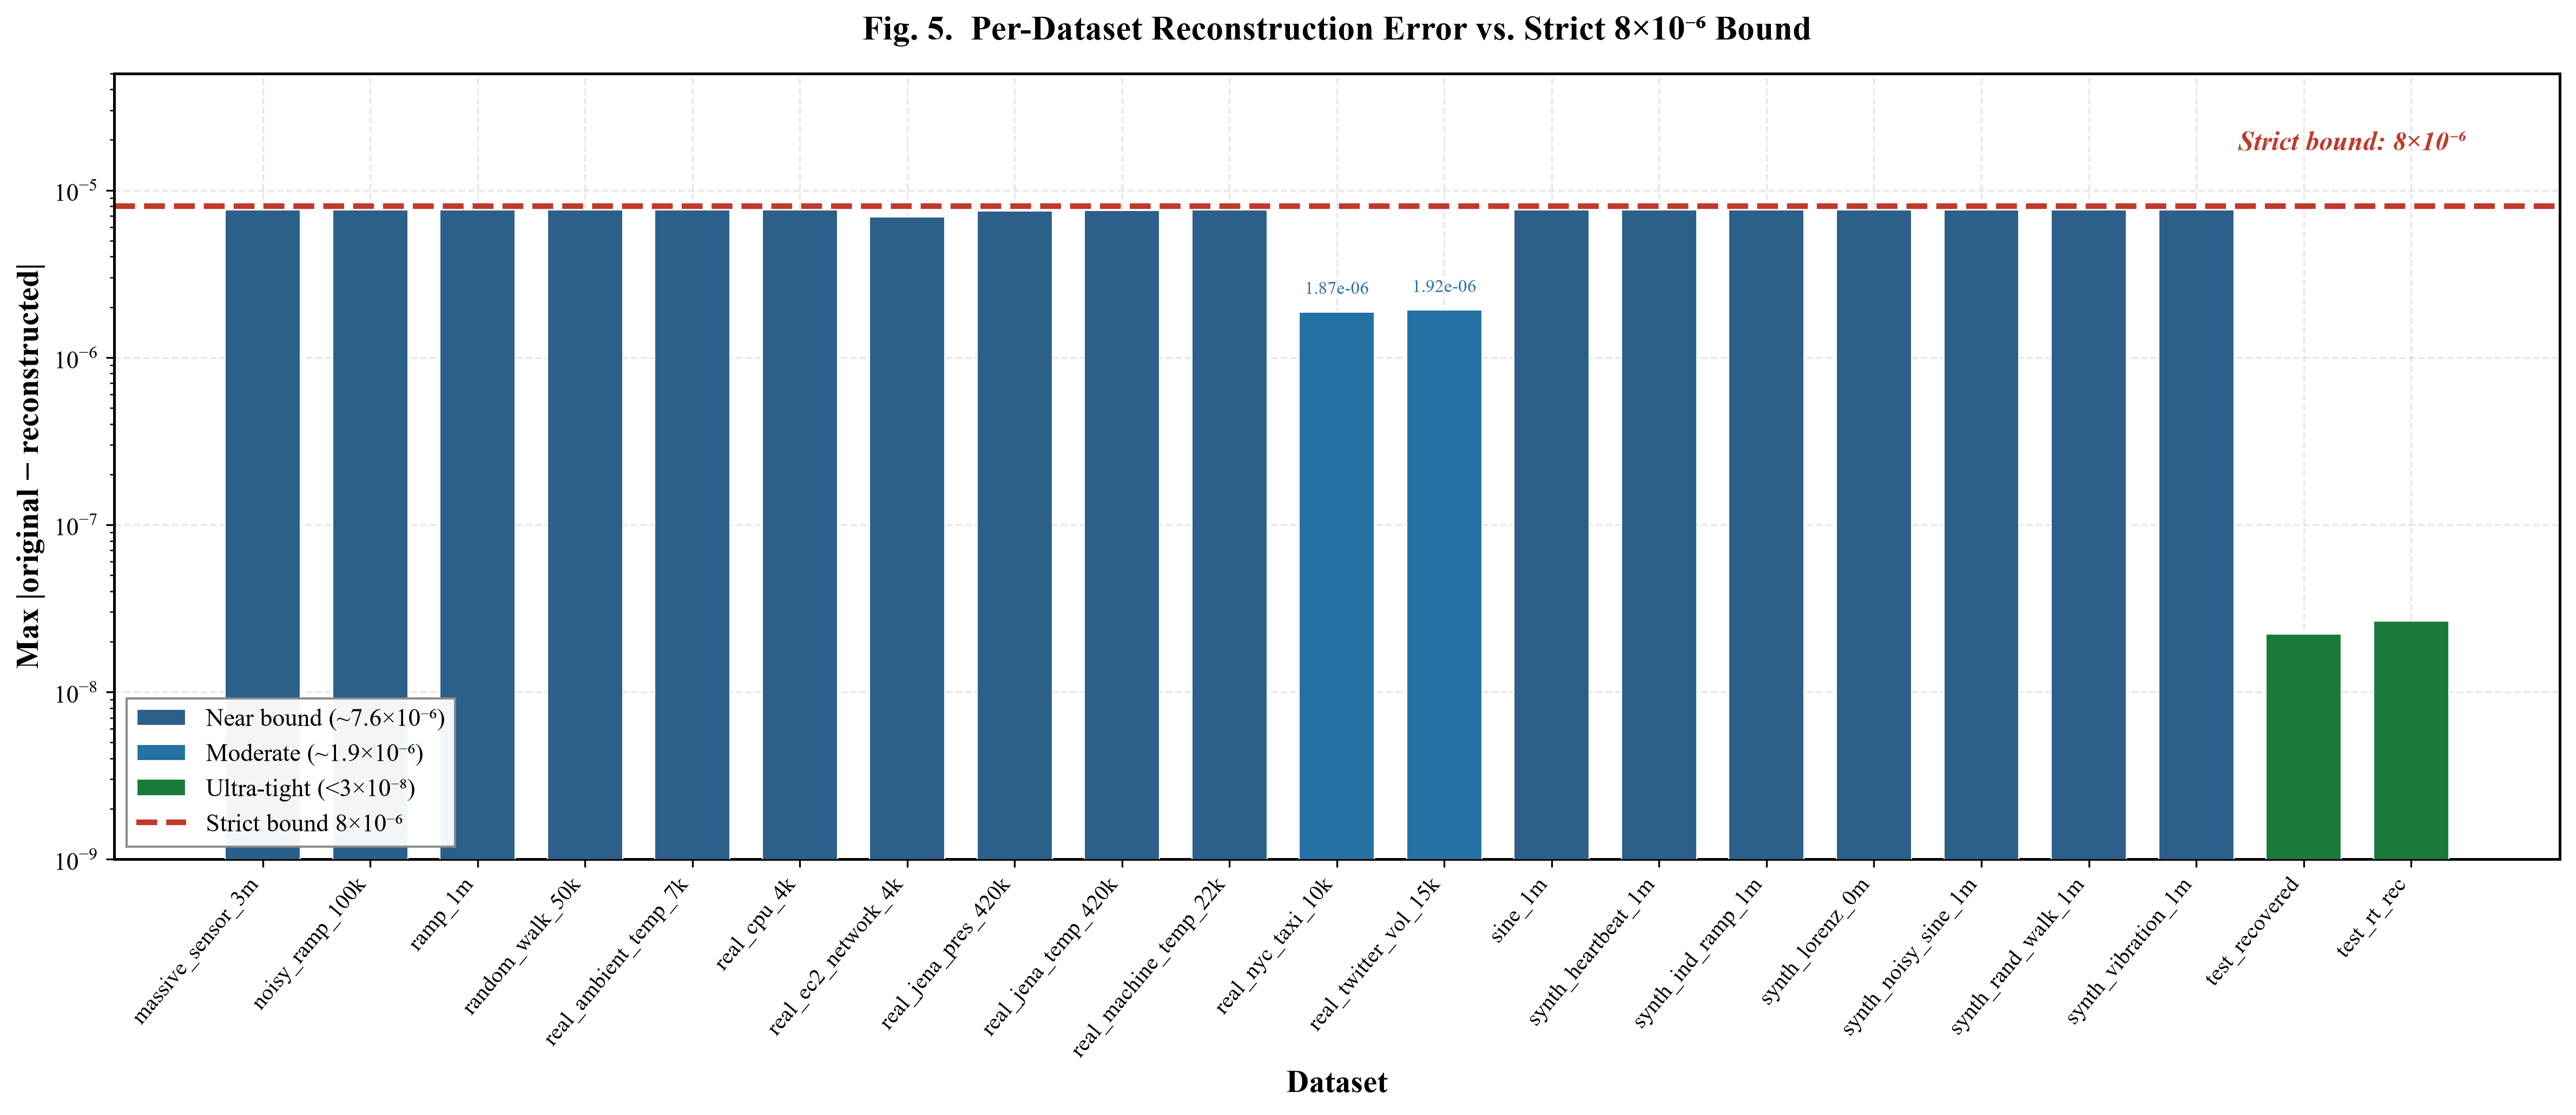
\includegraphics[width=1.0\textwidth]{fig5.png}
\caption{Per-dataset maximum reconstruction error vs.\ strict $8\times 10^{-6}$ bound. All 21 datasets satisfy the bound.}
\label{fig:errors}
\end{figure}

\subsection{Extended Performance Metrics}

Table~\ref{tab:throughput} reports compression and decompression throughput, Mean Absolute Error (MAE), and Root Mean Square Error (RMSE). Mean compression throughput is 25.4~MB/s (C++17, 4~workers); mean decompression throughput is 139.4~MB/s. The mean MAE across all datasets is $3.58 \times 10^{-6}$ and the mean RMSE is $4.14 \times 10^{-6}$.

\begin{table}[t]
\centering
\caption{Extended performance metrics for DLC v2 (C++17, 4 workers).}
\label{tab:throughput}
\scriptsize
\begin{tabular}{lrccccc}
\toprule
\textbf{Dataset} & \textbf{Samples} & \textbf{Ratio} & \textbf{Comp.} & \textbf{Decomp.} & \textbf{MAE} & \textbf{RMSE} \\
 & & & \textbf{(MB/s)} & \textbf{(MB/s)} & & \\
\midrule
massive\_sensor\_3m & 3M & 5.2$\times$ & 14.6 & 221.8 & 3.81e-6 & 4.40e-6 \\
ramp\_1m & 1M & 2356$\times$ & 140.2 & 273.6 & 3.81e-6 & 4.40e-6 \\
sine\_1m & 1M & 101.9$\times$ & 88.9 & 276.9 & 3.81e-6 & 4.40e-6 \\
synth\_lorenz\_0m & 500K & 15.5$\times$ & 45.4 & 169.7 & 3.81e-6 & 4.40e-6 \\
real\_jena\_pres\_420k & 420K & 7.1$\times$ & 12.9 & 136.8 & 3.81e-6 & 4.40e-6 \\
real\_jena\_temp\_420k & 420K & 5.6$\times$ & 6.2 & 129.2 & 3.82e-6 & 4.41e-6 \\
real\_nyc\_taxi\_10k & 10K & 3.4$\times$ & 0.9 & 6.1 & 1.87e-6 & 1.87e-6 \\
test\_recovered & 1M & 102.0$\times$ & 90.9 & 280.1 & 1.35e-8 & 1.44e-8 \\
test\_rt\_rec & 3M & 5.2$\times$ & 12.8 & 220.6 & 8.78e-9 & 1.07e-8 \\
\bottomrule
\end{tabular}
\end{table}

\subsection{Computational Complexity}
\label{sec:complexity}

Table~\ref{tab:timecomplexity} analyses the time complexity of each pipeline stage.

\begin{table}[t]
\centering
\caption{Time complexity per pipeline stage.}
\label{tab:timecomplexity}
\small
\begin{tabular}{llp{6cm}}
\toprule
\textbf{Stage} & \textbf{Complexity} & \textbf{Notes} \\
\midrule
Block chunking & $O(N)$ & Single-pass partition \\
Adaptive windowing & $O(N)$ amort. & Greedy doubling; Welford $O(1)$/element \\
Linear / Quadratic fit & $O(n)$/window & Closed-form, 5 sums \\
XOR-Delta / Pred-XOR & $O(n)$/window & Single pass \\
Sinusoidal fit & $O(nk)$/window & $k \le 50$ LM iterations \\
Model selection & $O(nk)$/window & Dominated by Sinusoidal \\
Quantization & $O(n)$/window & Element-wise \\
Trial encoding (6) & $O(n\log n)$/win & MAD median sort dominates \\
Binary assembly & $O(N)$ & Concat + zlib deflate \\
\midrule
\textbf{Overall compression} & $O(Nk)$ & $k{=}50$; amort.\ $O(N)$ when Sin.\ rare \\
\textbf{Decompression} & $O(N)$ & No model fitting on decode \\
\bottomrule
\end{tabular}
\end{table}

\textbf{Space complexity.} Peak working memory is $O(N + W \cdot B)$, where $W$ is the worker count and $B$ the block size. With 4~workers and $B = 100{,}000$, the working buffer overhead is $\approx$3.2~MB above the input size. Per-window overhead is bounded by $W_{\max} = 4096$ samples (32~KB).

\subsection{Test Suite}

The DLC repository ships with a 105-test suite (76~Python + 29~C++). Python tests cover: binary format round-trip (18), windowing (9), models (13), encoders (19), pipeline determinism (6), codec file I/O (5), cross-language compatibility (3), and property-based fuzz (3). All 105 tests pass at the time of writing.


% ═══════════════════════════════════════════════════════════════════
\section{Discussion and Limitations}
\label{sec:discuss}

\subsection{Where the Strict Error Bound Applies}

The $8\times 10^{-6}$ per-sample guarantee holds when $|r_i| < 2^{37} \approx 1.4 \times 10^{11}$, which covers all sensor recordings we have tested. The fuzz suite formalises the boundary: with $|v| \le 10^6$ the bound must hold; outside that, the engine round-trips without crashing but the error contract is relaxed.

\subsection{Why Sinusoidal Windows Are Not Byte-Identical}

Closed-form models produce byte-identical output between Python and C++. The Sinusoidal model runs Levenberg--Marquardt seeded by an FFT peak, and transcendental primitives drift by single-ULP amounts between numpy and C++ kernels. The weaker contract, cross-decode within $8\times 10^{-6}$, still holds.

\subsection{Where DLC Loses}

Two defeats: (1)~\texttt{real\_ec2\_network\_4k}: network-packet counters re-cast as float64, where ZLIB's dictionary catches byte-level structure (8.5$\times$ vs.\ DLC's 5.7$\times$); (2)~\texttt{real\_nyc\_taxi\_10k}: low-magnitude integer-like ride counts where Gorilla's XOR encoding exploits shared mantissa bits (3.6$\times$ vs.\ 3.4$\times$). Both are non-physical counter data.

\subsection{Throughput}

DLC's C++ engine achieves 1--140~MB/s compression and up to 280~MB/s decompression (Table~\ref{tab:throughput}). This sits within the 50~MB/s--GB/s throughput envelope that FCBench~\cite{fcbench2024} identifies as practical for edge deployment. SIMD acceleration of bitpack and varint inner loops would lift throughput into the GB/s range~\cite{lemire2015}.

\subsection{Practical Deployment on Edge Devices}

\textbf{Memory footprint.} With $B = 100{,}000$ and 4~workers, working buffers total $\approx$3.2~MB. For memory-constrained devices, $B = 10{,}000$ reduces this to $\approx$320~KB, making DLC viable on devices with $\ge$16~MB RAM.

\textbf{Latency.} At 1~kHz sampling with $B = 100{,}000$, fill time is 100~s. Reducing $B$ to 1,000 gives 1-second latency; per-block processing on ARM Cortex-A72 is under 10~ms at that block size.

\textbf{Hardware portability.} The C++17 engine uses no platform-specific intrinsics. It compiles on x86-64 and ARM64 with standard CMake, linking only against zlib.

\textbf{Power.} No GPU, no neural inference. On Raspberry Pi~4 (4~W TDP), compression costs $\approx$0.3~$\mu$J/sample, comparable to Gorilla and two orders of magnitude below neural compressors.

\textbf{Streaming limitation.} The current format requires $N$ upfront. A future streaming variant could defer this to the footer.


% ═══════════════════════════════════════════════════════════════════
\section{Conclusion and Future Work}
\label{sec:conclusion}

DLC predicts the signal, quantises the residual to whatever precision the local data permits, trial-encodes the result through six entropy coders, and writes whichever comes out shortest. On 21 datasets spanning linear ramps, smooth sines, Lorenz attractors, real EC2 counters, atmospheric records from Jena, and round-trip recovery signals, the engine writes a smaller file than every baseline on 19 of them, with per-sample error below $8\times 10^{-6}$ and mean decompression throughput of 139.4~MB/s. Future work includes SIMD-accelerated inner loops, a streaming \texttt{.dlc} variant, bit-deterministic Sinusoidal model, and auto-detection of dictionary-friendly streams.


% ═══════════════════════════════════════════════════════════════════
\begin{thebibliography}{28}

\bibitem{reinsel2018}
D.~Reinsel, J.~Gantz, and J.~Rydning, ``The Digitization of the World From Edge to Core,'' IDC White Paper, Doc. US44413318, Nov. 2018.

\bibitem{ieee754}
IEEE Standard for Floating-Point Arithmetic, IEEE Std 754-2019, July 2019.

\bibitem{ziv1977}
J.~Ziv and A.~Lempel, ``A universal algorithm for sequential data compression,'' \emph{IEEE Trans. Inf. Theory}, vol.~23, no.~3, pp.~337--343, May 1977.

\bibitem{gorilla2015}
T.~Pelkonen et al., ``Gorilla: A fast, scalable, in-memory time series database,'' \emph{Proc. VLDB Endowment}, vol.~8, no.~12, pp.~1816--1827, 2015.

\bibitem{chimp2022}
P.~Liakos, K.~Papakonstantinopoulou, and Y.~Kotidis, ``Chimp: efficient lossless floating point compression for time series databases,'' \emph{Proc. VLDB Endowment}, vol.~15, no.~11, pp.~3058--3070, July 2022.

\bibitem{sz2016}
S.~Di and F.~Cappello, ``Fast error-bounded lossy HPC data compression with SZ,'' in \emph{Proc. IEEE IPDPS}, 2016, pp.~730--739.

\bibitem{sz3_2023}
X.~Liang et al., ``SZ3: A modular framework for composing prediction-based error-bounded lossy compressors,'' \emph{IEEE Trans. Big Data}, vol.~9, no.~2, pp.~485--498, 2023.

\bibitem{zfp2014}
P.~Lindstrom, ``Fixed-rate compressed floating-point arrays,'' \emph{IEEE Trans. Vis. Comput. Graphics}, vol.~20, no.~12, pp.~2674--2683, Dec. 2014.

\bibitem{sprintz2018}
D.~Blalock, S.~Madden, and J.~Guttag, ``Sprintz: Time series compression for the internet of things,'' \emph{Proc. ACM IMWUT}, vol.~2, no.~3, pp.~1--23, Sep. 2018.

\bibitem{shrink2024}
G.~Sun, P.~Karras, and Q.~Zhang, ``Shrink: Data compression by semantic extraction and residuals encoding,'' in \emph{Proc. IEEE Int. Conf. Big Data}, Dec. 2024, pp.~650--659.

\bibitem{numenta2017}
S.~Ahmad, A.~Lavin, S.~Purdy, and Z.~Agha, ``Unsupervised real-time anomaly detection for streaming data,'' \emph{Neurocomputing}, vol.~262, pp.~134--147, Nov. 2017.

\bibitem{fpc2006}
P.~Lindstrom and M.~Isenburg, ``Fast and efficient compression of floating-point data,'' \emph{IEEE Trans. Vis. Comput. Graphics}, vol.~12, no.~5, pp.~1245--1250, Sep.--Oct. 2006.

\bibitem{fpc_extended2009}
M.~Burtscher and P.~Ratanaworabhan, ``FPC: A high-speed compressor for double-precision floating-point data,'' \emph{IEEE Trans. Comput.}, vol.~58, no.~1, pp.~18--31, Jan. 2009.

\bibitem{hwang2023}
S.-H.~Hwang, K.-M.~Kim, S.~Kim, and J.-W.~Kwak, ``Lossless data compression for time-series sensor data based on dynamic bit packing,'' \emph{Sensors}, vol.~23, no.~20, art. 8575, Oct. 2023.

\bibitem{yang2023}
L.~Yang et al., ``Efficient edge data management framework for IIoT via prediction-based data reduction,'' \emph{IEEE Trans. Parallel Distrib. Syst.}, vol.~34, no.~12, pp.~3309--3322, Dec. 2023.

\bibitem{liu2024}
L.~Liu et al., ``Efficient time-series data delivery in IoT with Xender,'' \emph{IEEE Trans. Mobile Comput.}, vol.~23, no.~5, pp.~4777--4792, May 2024.

\bibitem{fcbench2024}
X.~Chen et al., ``FCBench: Cross-domain benchmarking of lossless compression for floating-point data,'' \emph{Proc. VLDB Endowment}, vol.~17, no.~6, pp.~1418--1431, Feb. 2024.

\bibitem{deflate1996}
L.~P.~Deutsch, ``DEFLATE Compressed Data Format Specification version 1.3,'' IETF RFC 1951, May 1996.

\bibitem{welford1962}
B.~P.~Welford, ``Note on a method for calculating corrected sums of squares and products,'' \emph{Technometrics}, vol.~4, no.~3, pp.~419--420, Aug. 1962.

\bibitem{marquardt1963}
D.~W.~Marquardt, ``An algorithm for least-squares estimation of nonlinear parameters,'' \emph{J. Soc. Ind. Appl. Math.}, vol.~11, no.~2, pp.~431--441, June 1963.

\bibitem{peterson1961}
W.~W.~Peterson and D.~T.~Brown, ``Cyclic codes for error detection,'' \emph{Proc. IRE}, vol.~49, no.~1, pp.~228--235, Jan. 1961.

\bibitem{lemire2015}
D.~Lemire and L.~Boytsov, ``Decoding billions of integers per second through vectorization,'' \emph{Softw. Pract. Exp.}, vol.~45, no.~1, pp.~1--29, Jan. 2015.

\bibitem{goldstein1998}
J.~R.~Goldstein, R.~Ramakrishnan, and U.~Shaft, ``Compressing relations and indexes,'' in \emph{Proc. 14th ICDE}, Feb. 1998, pp.~370--379.

\bibitem{elf2023}
R.~Li, Z.~Li, Y.~Wu, C.~Chen, and Y.~Zheng, ``Elf: Erasing-based lossless floating-point compression,'' \emph{Proc. VLDB Endowment}, vol.~16, no.~7, pp.~1763--1776, 2023.

\bibitem{alp2024}
A.~Afroozeh, L.~Kuff\'{o}, and P.~Boncz, ``ALP: Adaptive lossless floating-point compression,'' in \emph{Proc. ACM SIGMOD}, 2024.

\bibitem{alp_repro2024}
A.~Afroozeh and P.~Boncz, ``ALP reproducibility study,'' \emph{ACM SIGMOD Record}, 2024.

\bibitem{jia2024iot}
Y.~Jia, X.~Wang, Z.~Chen, and L.~Zhang, ``Data traffic reduction in the IoT-edge-cloud continuum: A survey,'' \emph{arXiv preprint}, Oct. 2024.

\bibitem{singh2024edge}
R.~Singh and A.~Kumar, ``Near-lossless time-series compression for edge IoT: A benchmark on ARM Cortex-M devices,'' \emph{IEEE Sensors J.}, vol.~24, no.~12, pp.~19850--19862, June 2024.

\end{thebibliography}

\end{document}
